\section{Definizione dell'intervento di sistemazione e trasporto solido atteso}
Al fine di dimensionare le opere idrauliche da poter costruire all'interno del bacino idraulico, è necessario studiare le caratteristiche morfologiche del bacino stesso e del reticolo idraulico che lo attraversa.\\
Infatti, il processo erosivo prodotto dal reticolo idraulico dipende da:
\begin{itemize}
    \item tipologia del corso d'acqua alluvionale ed i suoi gradi di libertà (incisione ed allargamento);
    \item forma di trasporto solido prevalente: di fondo, iperconcentrato, colate detritiche,...;
    \item tipo di torrente: di scavo o di trasporto.
\end{itemize}
Il trasporto solido generato dalla corrente può essere:
\begin{itemize}
    \item ``bedload" (di fondo): comprende lo strisciamento, rotolamento o saltellamento dei sedimenti del letto del fiume;
    \item ``suspended load" (in sospensione): è generato dai vortici di turbolenza del flusso d'acqua, e trasporta generalmente il materiale di piccole dimensioni.
\end{itemize} 
\subsubsection{Equilibrio e dinamica del torrente}
Le modificazioni che si verificano in un corso d'acqua sono il risultato della sua tendenza a trovare uno stato di equilibrio.\\
Questo concetto può essere compreso considerando la ``Bilancia di Lane" (1955), ovvero una rappresentazione grafica che permette di capire come sarà il comportamento di un corso d'acqua al fine di raggiungere il proprio equilibrio.
\begin{figure}[H]  \centering
    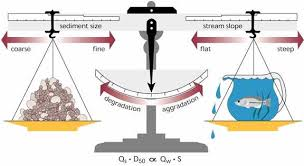
\includegraphics[scale=1]{immagini/bilancia_lane.jpg}
    \caption{Bilancia di Lane}
    \label{bilancia_lane}
\end{figure}
Matematicamente, il comportamento di un torrente al fine di ottenere l'equilibrio può essere riportato con questa formula:
\begin{equation}
    Q_L \cdot S \overset{=}{\propto} Q_S \cdot D_{50}
    \label{bilancia_lane}
\end{equation}
Dove:
\begin{itemize}
    \item $Q_L$ è la portata liquida del corso d'acqua;
    \item $S$ è la pendenza del thalweg;
    \item $Q_S$ indica la portata solida di sedimenti trasportata;
    \item $D_{50}$ indica il valore mediano della serie granulometrica rilevata nell'alveo.
\end{itemize}
La formula \ref{bilancia_lane} può anche essere considerata come se al primo membro fosse rappresentata la ``stream power" del fiume ed al secondo membro fosse riportato l'attrito al movimento.\\
Secondo la ``Classificazione di Horatiis" (1930), i tratti fluviali di montagna possono essere suddivisi in:
\begin{itemize}
    \item torrenti di trasporto: l'energia della corrente è tale da essere completamente impegnata nel trasporto di materiale solido a valle; il letto tende a non abbassarsi o ad alzarsi. Le opere progettate per questi tratti hanno l'obiettivo di trattenere il sedimento;
    \item torrenti di scavo: l'energia della corrente produce trasporto solido ed incisione del letto; il letto tende ad abbassarsi, generando una tendenza all'incisione verso monte. Le opere progettate per questi tratti hanno l'obiettivo di consolidare maggiormente i tratti dove l'opera di erosione ha una maggiore presenza.
\end{itemize}

\subsection{Briglie di consolidamento}
Mediante le briglie di consolidamento si vuole indurre il tratto di reticolo verso una pendenza di equilibrio dinamico del profilo ($i_c$) \ref{profilo_briglia_consolidamento}.\\
La pendenza $i_c$ equivale alla pendenza che è necessario assegnare ad un certo tratto fluviale, affinché si trovi nelle condizioni di mettere in mobilità una precisa quantità granulometrica di sedimento al fondo.\\
Le briglie di consolidamento possono essere di tipo longitudinale (per la stabilizzazione delle sponde) o di tipo trasversale (al fine di ridurre o controllare la pendenza longitudinale del profilo.)
In molti casi, se necessario, vengono erette in successione una serie di briglie di consolidamento.

\begin{figure}[H] \centering
    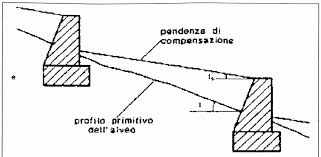
\includegraphics[scale=1]{immagini/profilo_briglia_consolidamento.jpg}
    \caption{Profilo di una briglia di consolidamento, con riportata la pendenza originaria e quella che si manifesta successivamente alla costruzione dell'opera.}
    \label{profilo_briglia_consolidamento}
\end{figure}

Il dimensionamento ed ulteriori informazioni su queste opere idrauliche verranno riportate più approfonditamente nel capitolo successivo.

\subsection{Studio della granulometria}
Con il termine ``granulometria" s'intende la proprietà con cui è possibile descrivere e studiare un insieme di particelle del suolo, siano queste sabbiose, ghiaiose,...\\
Lo studio granulometrico permette di conoscere, in modo statistico, la composizione del terreno di studio.\\
L'analisi granulometrica inizia andando a misurare, in modo sistematico, la grandezza (generalmente il diametro) dei clasti presenti nel letto dell'alveo o nelle barre.\\
Successivamente, si procede alla suddivisione in classi dei diametri misurati, per poi andare a calcolare la frequenza relativa, cumulata e percentuale per ognuna.\\
Per il caso di studio di questa relazione, la curva che interpola la frequenza cumulata e la classe diametrica dei sedimenti è la seguente.
\begin{figure}[H] \centering
    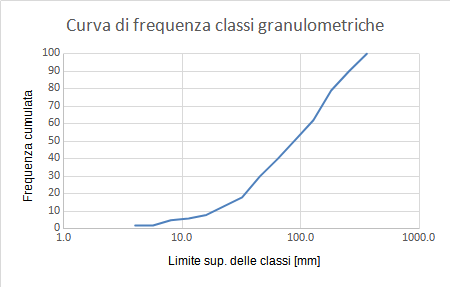
\includegraphics[scale=0.75]{immagini/curva_freq_classi_granuometriche.png}
    \caption{Curva della frequenza cumulata delle classi granulometriche.}
    \label{curva_freq_classi_granulometriche}
\end{figure}
Infine, per conoscere la distribuzione statistica delle grandezze dei  sedimenti, all'interno del campione rilevato, è necessario applicare la seguente formula:
\begin{equation}
D_\% = \left[\frac{D_2-D_1}{F_2-F_1}\right] \cdot (F-F_1)+D
\end{equation} 
Dove:
\begin{itemize}
    \item $D$ indica la classe diametrica;
    \item $F$ indica la frequenza cumulata.
\end{itemize}
Per il caso di studio inerente a questa relazione, i risultati sono:
\begin{table}[H]\centering
    \caption{\textcolor{red}{Classi di frequenza cumulata inerente ai sedimenti del bacino idrografico di studio. I valori relativi ai diametri sono espressi in $mm$.}}
    \begin{tabular}{cc}
    \toprule
    N   & 100      \\
    \midrule
    D16 & 28.25    \\
    D50 & 88.10    \\
    D84 & 215.10   \\
    D90 & 256.00   \\
    \bottomrule
    \end{tabular}
    \end{table}

\subsection{Calcolo della pendenza di correzione}
\subsubsection{Approccio statico per la stima di $i_c$}
Secondo Fattorelli et al. (1980), basandosi su 1000 tratti sistemati in Trentino, il valore $i_c$ può essere calcolato mediante le seguenti formule:
\begin{itemize}
    \item per bacini mediamente erodibili:
\begin{equation}
    i_c = 0.66 \cdot i_0 
\end{equation}
\item per bacini poco erodibili
\begin{equation}
    i_c = 0.77 \cdot i_0 
\end{equation}
\item per bacini molto erodibili
\begin{equation}
    i_c = 0.59 \cdot i_0 
\end{equation}
\end{itemize}
 
Secondo Heede (1960), il calcolo di $i_c$ avviene mediante:
\begin{equation}
    i_c = (0.6 - 0.7) \cdot i_0
\end{equation}

\subsubsection{Approccio mediante lo sforzo tangenziale medio}
Considerando le condizioni di moto uniforme ($i_F=i_E=i$), la corrente esercita sul contorno uno sforzo tangenziale medio, con formula:
\begin{equation}
    \tau = \gamma \cdot R_H \cdot i
\end{equation}
Conoscendo la $i_c$, ovvero la pendenza che si ambisce ad ottenere successivamente alla costruzione dell'opera, è possibile calcolare la $\tau_{c}$, mediante la formula precedentemente riportata.\\
Lo sforzo massimo che si genera nel letto del fiume, ha valore calcolabile mediante la formula:
\begin{equation}
    \tau_{max} = \gamma \cdot y \cdot i
\end{equation}
Mentre, per quanto riguarda lo sforzo agente sulle sponde, il calcolo avviene mediante:
\begin{equation}
    \tau_{sponde-fondo-max}= K \cdot (\gamma, y, i)
\end{equation}
Secondo le ricerche Shields (1936), e successive semplificazioni, la relazione tra sforzo al fondo e grandezza dei sedimenti è regolata dalla formula:
\begin{equation}
    \tau_c \approx 1000 \cdot D
\end{equation}
\subsubsection{Approccio deterministico per la stima di $i_c$}
Secondo Shields (1936), la formula per il calcolo dello sforzo tangenziale critico è:
\begin{equation}
    \tau_c = 0.06 \cdot (\gamma_s -\gamma) \cdot D
\end{equation}
Dove:
\begin{itemize}
   \item $D$ è la taglia granulometrica di riferimento;
    \item $\gamma_s$ è il peso specifico dei sedimenti;
    \item $\gamma$ è il peso specifico dell'acqua.
\end{itemize}
Tale formula può anche essere riscritta, diventando:
\begin{equation}
    i_c = \frac{\tau_c^* \cdot (\gamma_s-\gamma) \cdot D}{\gamma \cdot Rh}
\end{equation}

\subsubsection{Soluzione esplicita semplificata per sezioni rettangolari molto larghe}
